\chapter{基于问题分解的多跳长文本阅读理解}
% 摘要:SeqDecomposer, StepDecomposer
% 什么是多跳阅读理解
多跳机器阅读理解是指利用多个相关文档段落进行多次推理,以实现对复杂问题的理解和回答。
与常规的单跳机器阅读理解相比,多跳机器阅读理解需要综合运用文本中的信息、常识和推理能力。
% 多跳阅读理解一般用到什么技术
通常,多跳阅读理解使用基于图神经网络的方法或基于检索的方法。
其中,图卷积网络、图注意力网络和图循环网络通过邻接矩阵建立文档间多个句子或实体之间的联系。
基于检索的方法类似于第三章提到的方法,利用文本匹配模型得到与问题相关的文档,然后进行阅读理解。
% 这些技术的缺点
然而,这些模型不擅长寻找支持证据,因为它们缺乏进行真正的多跳推理的能力。
目前的多跳阅读理解模型往往是利用快捷方式进行求解,这意味着模型无需实际执行必要的推理步骤即可回答问题。
% 本文提出了什么方法,及其大致步骤
因此,本文提出了两种相关方法SeqDecomposer和StepDecomposer,用来将复杂的多跳问题分解为多个简单的单跳问题。
这些单跳问题依次检索相关文档作为支持证据,并对这些文档进行阅读理解,以获取每个子问题以及最终的答案。
% 本文提出了什么方法,及其大致步骤
本章在多跳阅读理解数据集MuSiQue上进行了实验。
实验结果表明,SeqDecomposer和StepDecomposer与现有的检索式基线模型相比,在支持证据F1的性能上取得了不错的提升。
因此,这两种方法可以更好地处理复杂的多跳问题,提高多跳阅读理解的性能。

\section{引言}
% 介绍多跳阅读理解
多跳阅读理解\cite{Yang2018HotpotQAAD}(Multi-hop Reading Comprehension,MH-RC)是指需要在多个相关文档段落中进行多次推理,以实现对复杂问题的理解和回答。
相较于单跳阅读理解,多跳阅读理解更接近于人类的语言推理能力,具有广泛的应用前景,但也具有极大的挑战性。
图~\ref{tab:5-1}~给出了一个多跳阅读理解数据集MuSiQue的例子。
例如,对于一个多跳问题“Who is the president of ... ?”,需要将其分解为四个子问题,每个子问题都不存在多跳的复杂关系。
对于每个单跳问题,需要在给定的文档集合中找到对应的文档,并从文档中抽取答案。
在该示例中,每个子问题的答案又会重新作用于下一个问题。
% 多跳阅读理解是一项重要的研究课题。它不仅能够解决传统单跳阅读理解任务中存在的问题,还能够应用于实际生活中更加复杂的场景,例如在医疗领域中,需要对多个医学文献进行分析才能得出正确的诊断结果。
% 因此,多跳阅读理解具有广阔的应用前景。

% 多跳阅读理解的一般方法及其缺点
在多跳推理中,系统需要利用多个文档中获取的信息进行推理,以得出最终答案。
然而,多跳阅读理解不仅需要获取最终答案,还需要系统筛选出可用于回答答案的支持文档。

\begin{table}[htbp]
    \centering
    \begin{tabular}{p{420pt}}
    \hline
    {\bfseries 相关文档:} \\
    文档13: BULLET::::- On 4 March 2006, Lion Air Flight 8987, a McDonnell Douglas MD-82, crashed after landing at Juanda International Airport. Reverse thrust was used during landing, although the left thrust reverser was stated to be out of service. This caused the aircraft to veer to the right and skid off the runway, coming to rest about from the approach end of the runway. There were no fatalities, but the aircraft was badly damaged and later written off. \\
    <译文:Aga Kagans会奴役Boyars> \\
    文档3: Cathay Pacific Flight 780 was a flight from Surabaya Juanda International Airport in Indonesia to Hong Kong International Airport on 13 April 2010. There were 309 pass       engers and a crew of 13 on board. As Flight 780 neared Hong Kong the crew were unable to change the thrust output of the engines. The aircraft, an Airbus A330-342, landed at almost twice the speed of a        normal landing, suffering minor damage. The 57 passengers who sustained injuries were hurt in the ensuing slide evacuation; one of them received serious injuries. \\
    <译文:Boyars和Aga Kagans会引发战争 > \\
    文档14: The Indonesia\u2013Timor Leste Commission on Truth and Friendship was a truth commission established jointly by the governments of Indonesia and East Timor in August 2       005. The commission was officially created to investigate acts of violence that occurred around the independence referendum held in East Timor in 1999 and sought to find the \"conclusive truth\" behind        the events. After holding private hearings and document reviews, the commission handed in the final report on July 15, 2008 to the presidents of both nations, and was fully endorsed by Indonesian Presid       ent Susilo Bambang Yudhoyono, providing the first acknowledgement by the government of Indonesia of the human rights violations committed by state institutions in Timor. The commission is notable for be       ing the first modern truth commission to be bilateral. \\
    <译文:Aga Kagans会离开Flamme,找到更好的星球> \\
    文档11: Democratic Republic of Timor - Leste Rep\u00fablika Demokr\u00e1tika Tim\u00f3r Lorosa'e (Tetum) Rep\u00fablica Democr\u00e1tica de Timor - Leste (Portuguese) Flag Coa       t of arms Motto: Unidade, Ac\u00e7\u00e3o, Progresso (Portuguese) Unidade, Asaun, Progresu (Tetum) (English: ``Unity, Action, Progress '') Anthem: P\u00e1tria (Portuguese) (English:`` Fatherland'') Capi       tal and largest city Dili 8 \u00b0 20 \u2032 S 125 \u00b0 20 \u2032 E \ufeff / \ufeff 8.34 \u00b0 S 125.34 \u00b0 E \ufeff / - 8.34; 125.34 Coordinates: 8 \u00b0 20 \u2032 S 125 \u00b0 20 \u2032 E \ufef       f / \ufeff 8.34 \u00b0 S 125.34 \u00b0 E \ufeff / - 8.34; 125.34 Official languages Tetum Portuguese National languages 15 languages (show) Atauru Baikeno Bekais Bunak Fataluku Galoli Habun Idalaka Kawa       imina Kemak Makalero Makasae Makuva Mambai Tokodede Religion (2010) 96.9\% Roman Catholic 3.1\% other religions Demonym East Timorese Timorese Maubere (informal) Government Unitary semi-presidential const       itutional republic President Francisco Guterres Prime Minister Mari Alkatiri Legislature National Parliament Formation Portuguese Timor 16th century Independence declared 28 November 1975 Annexation by        Indonesia 17 July 1976 Administered by UNTAET 25 October 1999 Independence restored 20 May 2002 Area Total 15,410 km (5,950 sq mi) (154th) Water (\%) negligible Population 2015 census 1,167,242 Density 7       8 / km (202.0 / sq mi) GDP (PPP) 2017 estimate Total \$4.567 billion Per capita \$5,479 (148th) GDP (nominal) 2014 estimate Total \$2.498 billion Per capita \$3,330 HDI (2015) 0.605 medium 133rd Currency Un       ited States Dollar (USD) Time zone (UTC + 9) Drives on the left Calling code + 670 ISO 3166 code TL Internet TLD. tl Website timor-leste.gov.tl Fifteen further ``national languages ''are recognised by t       he Constitution. Centavo coins also used.. tp has been phased out. \\
    <译文:Boyars会与Aga Kagans签订条约,而不需要得到Corps的批准> \\
    \hline
    {\bfseries 问题:} \\
    Who is the president of the newly declared independent country, that established the Timor Leste Commission of Truth and Friendship, with the country containing the airport that includes Lion Air? \\
    <译文:如果Corps不介入Boyars和Aga Kagans的争端,根据Retief的说法会发生什么? > \\
    \hline
    {\bfseries 问题分解:} \\
    子问题1: What airport is Lion Air part of? \\
    <译文:Aga Kagans会奴役Boyars> \\
    答案:Juanda International Airport \\
    子问题2: \#1 >> country \\
    <译文:Boyars和Aga Kagans会引发战争 > \\
    答案:Indonesia \\
    子问题3: #2 \u2013Timor Leste Commission of Truth and Friendship >> country \\
    <译文:Aga Kagans会离开Flamme,找到更好的星球> \\
    答案:East Timor \\
    子问题4: who is the president of newly declared independent country #3 \\
    <译文:Boyars会与Aga Kagans签订条约,而不需要得到Corps的批准> \\
    答案:Francisco Guterres \\
    \hline
    \end{tabular}
    \caption{\label{tab:5-1}
    MuSiQue中的例子。
    }
\end{table}


针对多跳阅读理解,通常可以采用两种不同的方法进行处理。
% HGN
其中一种方法是基于图神经网络,例如HGN\cite{Fang2019HierarchicalGN}(Hierarchical Graph Network)系统。
该系统使用一个层次化的图神经网络来执行多跳推理。
通过构建一个层次图来聚合来自多个段落的线索,该图由不同粒度级别(问题、段落、句子、实体)的节点构成。
该系统的表示形式使用预训练的BERT模型初始化。
% SAE
另一种方法是基于检索的方法,例如SAE\cite{Tu2019SelectAA}(Select, Answer and Explain)系统。
该系统通过使用一个可解释的模型来选择最相关的文档,然后在这些文档中执行多跳推理,以回答问题。

然而,这两种方法都存在一些问题。
尽管图神经网络能够直接找到答案,但其采用的黑盒模型无法提供充分的证据支持,因为它可以在不执行必要的推理步骤的情况下回答问题。
相比之下,检索的方式则采用了长文本阅读理解的做法,但未能充分利用多跳的特点。

% 本文提出的方法介绍
因此,本章使用人类回答多跳问题的方法,提出了一种基于问题分解的方法,将复杂的多跳问题分解为多个简单的单跳问题。
对于这些单跳问题,我们依次从长文本中检索出相关文档作为支持证据,并对这些文档进行阅读理解,以获取每个子问题的答案和最终答案。
% 实验性能
本章在MuSiQue多跳阅读理解数据集上对两种问题分解方法SeqDecomposer和StepDecomposer进行了实验。
实验结果显示,相较于现有的检索式基线模型,本章提出的方法在支持证据F1评价指标上有显著提升。

% 主要贡献
本章的主要贡献如下:
\begin{itemize}
    \item[$\bullet$] 针对多跳阅读理解领域,本章采用问题分解的基本思路,提出了SeqDecomposer和StepDecomposer两种方法。这些方法通过将复杂的多跳问题分解为多个简单的单跳问题,更好地适应了阅读理解任务。
    \item[$\bullet$] 本章采用生成式模型对抽取式阅读理解任务中的问题分解部分进行评价,并评估了多跳问题的分解效果。
    \item[$\bullet$] 本章针对多跳阅读理解数据集MuSiQue,展示了SeqDecomposer和StepDecomposer方法相对于检索式基线模型在支持证据F1上的明显提升。
\end{itemize}


\section{基于问题分解的多跳长文本阅读理解}
本节提出了一个基于问题分解来完成多跳阅读理解的模型架构SeqDecomposer。
本节将按照SeqDecomposer的问题分解部分,检索与阅读理解部分,以及对其进行的改善三方面进行逐一展开。
% 首先,本节将重点介绍SeqDecomposer的问题分解模块。
% 在完成问题分解后,SeqDecomposer模型将利用预训练语言模型来进行阅读理解。
% 最后,本节还提出了一个全新的StepDecomposer架构,用于进一步改善SeqDecomposer模型的性能。

\subsection{总体架构}
% 介绍框架
图~\ref{fig:5-1}展示了本章提出的SeqDecomposer模型的结构,它由三个主要组成部分构成。
% 问题分解部分
首先,问题分解模块使用流行的序列到序列生成网络将复杂的多跳问题分解为多个简单的单跳问题。
% 检索和阅读部分
然后,基于神经网络的检索模型和阅读理解模型将生成模型得到的单跳问题与文档集合并,得出问题的答案,并将答案与下一个问题进行充分的结合,得到下一步骤的完整表示。
% 如何把两个模块统一起来
最后,本文对SeqDecomposer模型进行了改进,得到了新的StepDecomposer架构,该架构多次执行问题分解过程,并将生成结果传递给检索和阅读模型。

% 整体任务结构
\begin{figure}[htbp]
    \centering
    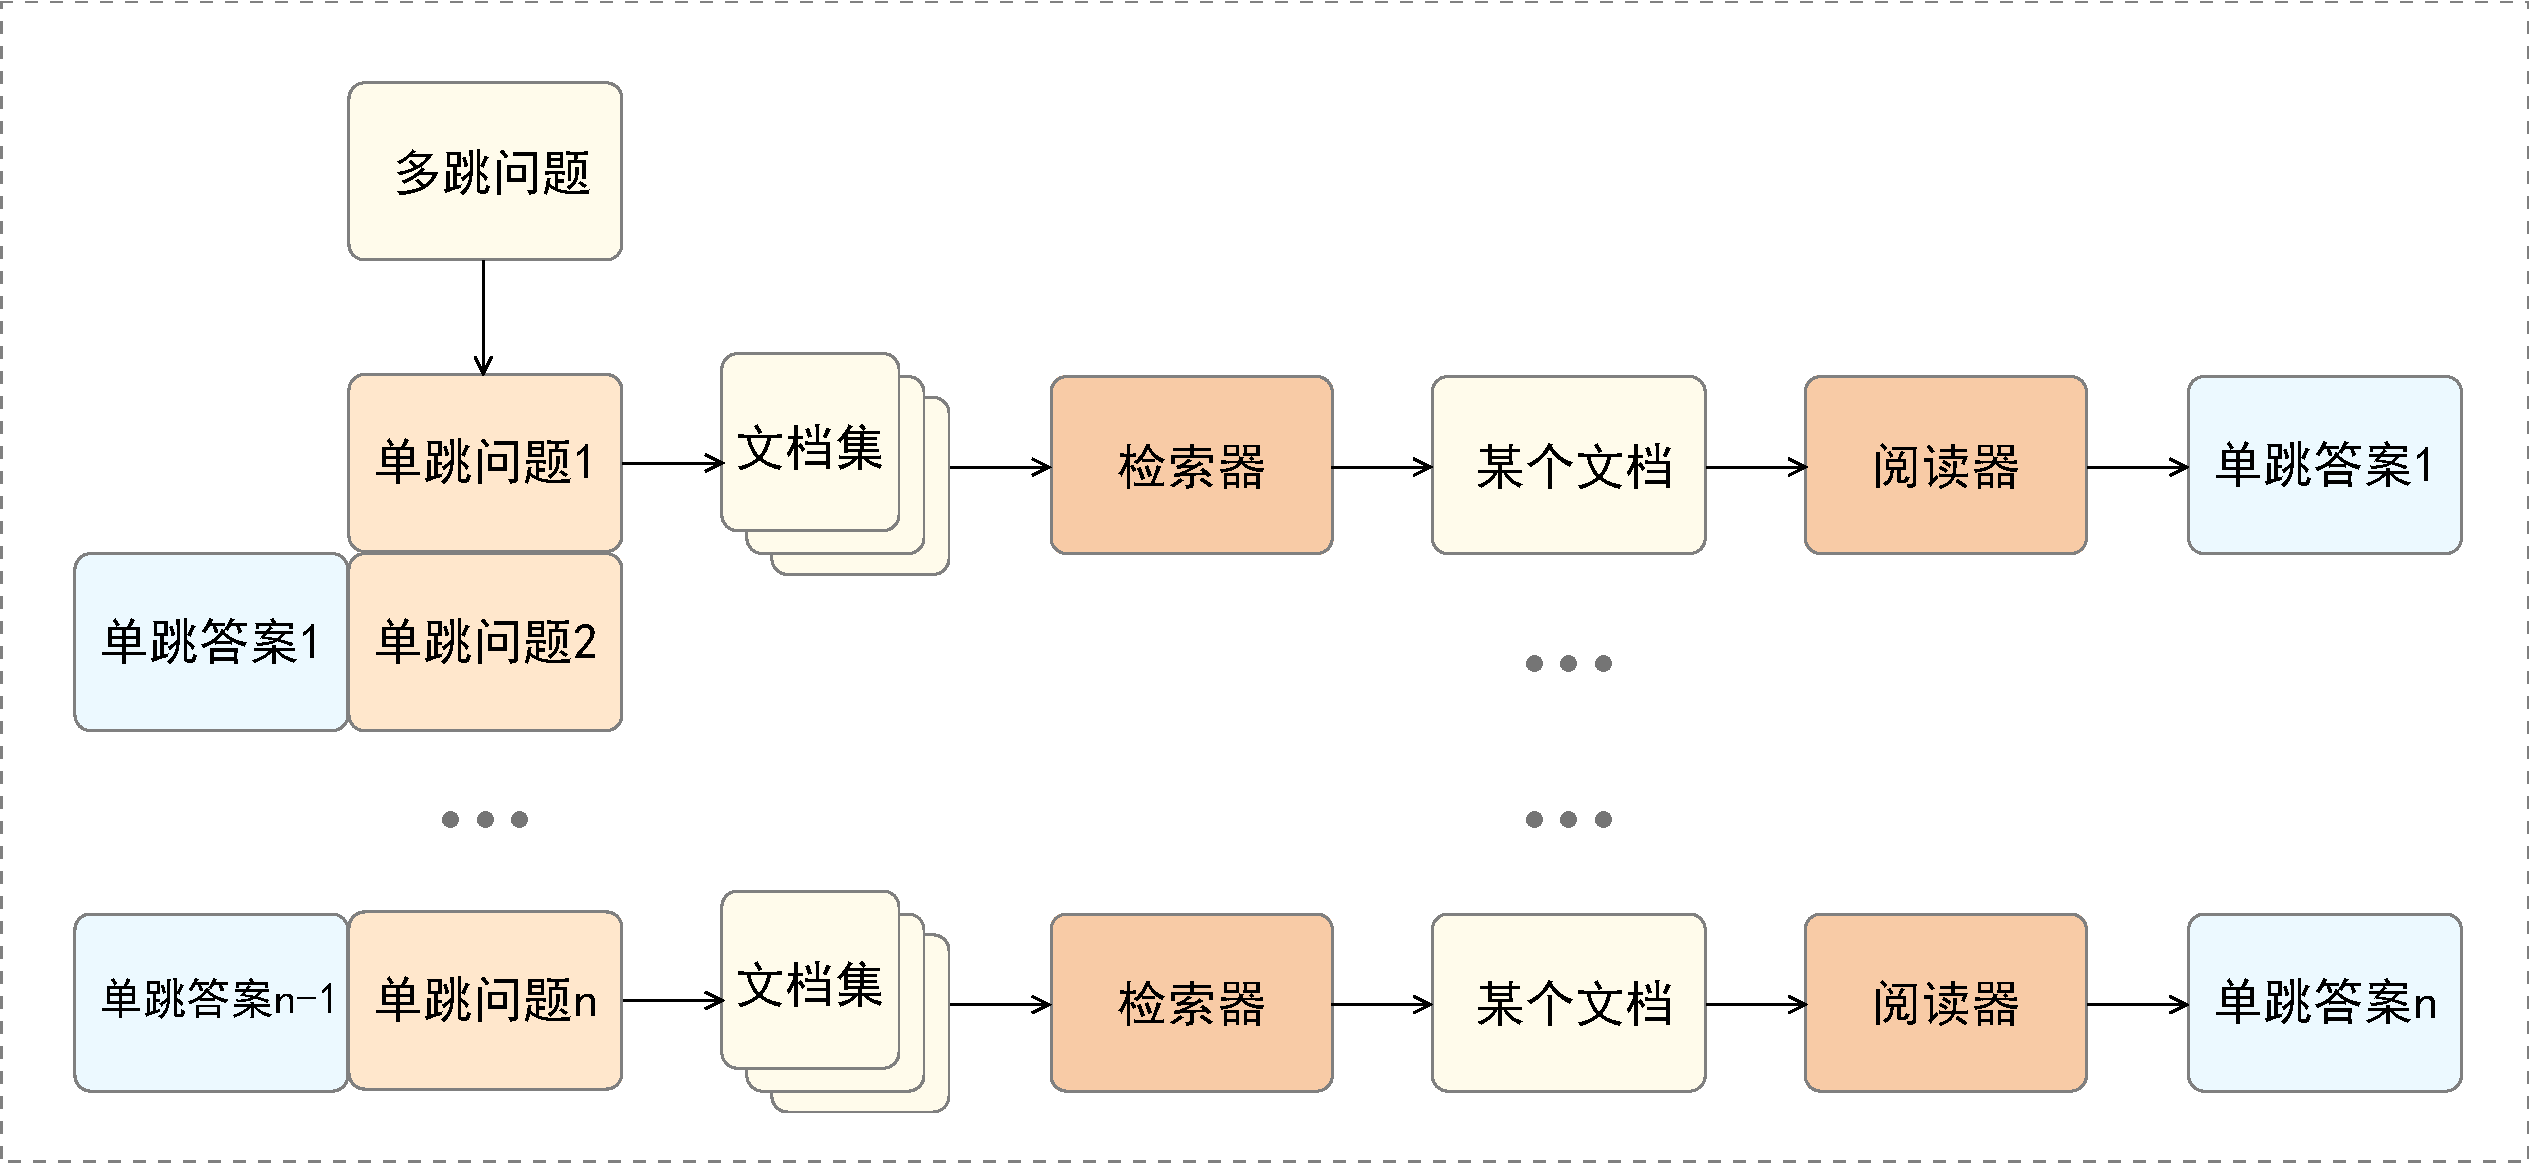
\includegraphics [width=1.0\textwidth] {figure/5-1.pdf}
    \caption{SeqDecomposer的整体架构} 
    \label{fig:5-1}
\end{figure}


\subsection{基于序列到序列生成的问题分解模块}
% 为什么要使用问题分解技术?
问题分解技术是一种将复杂多跳问题分解成多个简单单跳问题的方法。
这种方法的优点在于简化了问题的回答过程,使得回答过程更加可控和可解释。

% 怎么做的
本文提出了SeqDecomposer架构,该架构采用序列到序列的生成模型,对于多跳问题$Q$,将其分解为多个单跳问题$q_1,q_2,...,q_n$。
这个过程可以表示为:
\begin{equation}
    q_1,q_2,...,q_n = GEN(Q)
\end{equation}
序列到序列的生成模型通常包括BART和T5等。
BART\cite{Lewis2019BARTDS}(Bidirectional and Auto-Regressive Transformer)是Facebook AI Research在2019年提出的一种序列到序列的生成模型,具有自编码和自回归的能力,能够在不同的任务中共享参数。
而T5\cite{Ni2021SentenceT5SS}(Text-to-Text Transfer Transformer)是Google在2020年提出的一种序列到序列的生成模型,可以将所有的自然语言处理任务都转化为文本到文本的转换任务,从而用同一种模型解决不同的任务。
在本文中,同时使用了BART和T5来进行相关实验比较。
需要注意的是,从生成第二个及以后的子问题$q_i(i\geq 2)$开始,由于$q_i$可能需要前一个子问题$q_{i-1}$的答案$a_{i-1}$,因此在生成子问题$q_i$时,需要先将先前的答案$a_{i-1}$以词槽的形式填充到子问题$q_{i-1}$中。
直到整个系统得到最后一个子问题$q_{n}$的答案$a_{n}$后,将停止迭代。

\subsection{基于预训练语言模型的阅读理解模型}
% 浅谈检索和阅读理解
在多跳阅读理解中,通常会以多文档的形式提供参考文本。
这种形式导致文本总长度通常会非常长。
因此,与第三章类似,本章需要针对每个单跳问题进行文档检索和阅读的操作。

% 如何检索单跳问题的相关文档
针对单跳问题$q_i$,需要先进行检索,从备选文档中找到相关文档。
在MuSiQue数据集中,大部分问题都分配到20个文档,记为$D={D_1, D_2, ..., D_20}$,这20个文档只有一个与$q_i$相关。
为了进行检索,可以将子问题$q_i$与所有文档依次拼接,形成$x_{ij}=[CLS]q_i[SEP]D_j[SEP]$。通过一个预训练语言模型,可以得到$x_{ij}$的整体表示$H_{ij}$。
接着,使用一层全连接网络和Softmax层计算$H_{ij}$的分类概率值$\hat y_c$,表示子问题$q_i$与文档$D_j$的相关性。
损失函数可以计算$\hat y_{ij}$与子问题$q_i$对应的正确文档标签$y_{ij}$之间的差距,以监督检索模型的学习。
其中,检索出与子问题$q_i$相关的文档的交叉熵损失函数可以表示为:
\begin{equation}
    \mathcal  L^{Retr}_{i}  = -y_{ij}\log\hat y_{ij}+(1-y_{ij})log(1-\hat y_{ij})
\end{equation}

% 如何抽取单跳问题的答案
在得到子问题$q_i$相关的文档$D_j$后,阅读模块需要将两者的表示拼接在一起,得到$x_i=[CLS]q_i[SEP]D_j[SEP]$。
然后,阅读模块中的编码器将$x_i$转化成隐向量;
该隐向量经过一个指针网络,可以标识出文档中每个token作为答案起始位置和结束位置的概率值,分别用$\hat{y_s}$和$\hat{y_e}$来表示。
训练过程中,用真实答案的起始和结束位置$y_s$和$y_e$来进行训练,其损失函数可以表示为:
\begin{equation}
    \mathcal L^{Ans}_{i} = \frac{1}{2} CrossEntropy(\hat y_s,y_s) + \frac{1}{2} CrossEntropy(\hat y_e,y_e)
\end{equation}

% 如何将子答案融入到下一个单跳问题中
在推理阶段,若上述模型获取的子答案$a_i$不是最后一跳问题的答案,需将其填充至下一个单跳问题$q_{i+1}$中的槽位,以完成下一跳问题的形成。
这样,下一跳问题$q_{i+1}$即成为了一个完整的自然语言问题,可以不断循环执行检索与阅读的步骤,直到获取最终答案$a_n$为止。
% 这一过程能够提升模型的准确性和鲁棒性,增强其在问答任务中的表现。

\subsection{采用分步执行的问题分解技术}
% 前面的问题分解模式有什么缺点?为什么要改进?
在前文中提到的SeqDecomposer架构中,使用了序列到序列的生成模型,将复杂的多跳问题一次性分解为了一系列单跳问题。
虽然用占位符填充子问题可以使每个问题看起来具备连贯性,但本文认为在生成子问题的过程中,没有充分利用可用的答案信息。

% 新的问题分解的做法
为了改进SeqDecomposer的工作流程,本节提出了一种新的架构StepDecomposer,该架构针对问题分解部分进行了修改。
在处理复杂的多跳问题$Q$时,StepDecomposer的方法是每次只让生成模型生成一个单跳问题$q_i$,与SeqDecomposer相比,其具体实现方式有所不同。
具体实现过程如图~\ref{fig:5-2}~所示,对于问题Q以及已经生成的前$k-1$跳单跳问题$q_1, q_2, ..., q_{k-1}$,这些单跳问题已经通过前述的检索和阅读理解模型得到了对应的子答案$a_1, a_2, ..., a_{k-1}$。
此时,将这些已知信息,包括原始问题$Q$、单跳问题$q_1, q_2, ..., q_{k-1}$以及单跳答案$a_1, a_2, ..., a_{k-1}$输入到生成式模型中,目的是生成下一跳问题$q_k$,即:
\begin{equation}
    q_k = GEN(Q,q_1,a_1,q_2,a_2,...,q_{k-1},a_{k-1})
\end{equation}
完成最后一跳问题$q_n$的生成后,需要使用检索模型和阅读理解模型得到最终答案,以完成整个流程。
需要注意的是,现实应用中多跳问题的跳数是未知的。
因此,本文针对QuALITY训练集中的最后一跳问题添加了结束标记,以便在生成式模型生成带有结束标记的问题时,能够判断此时已经到达了最后一跳问题。

% 整体任务结构
\begin{figure}[htbp]
    \centering
    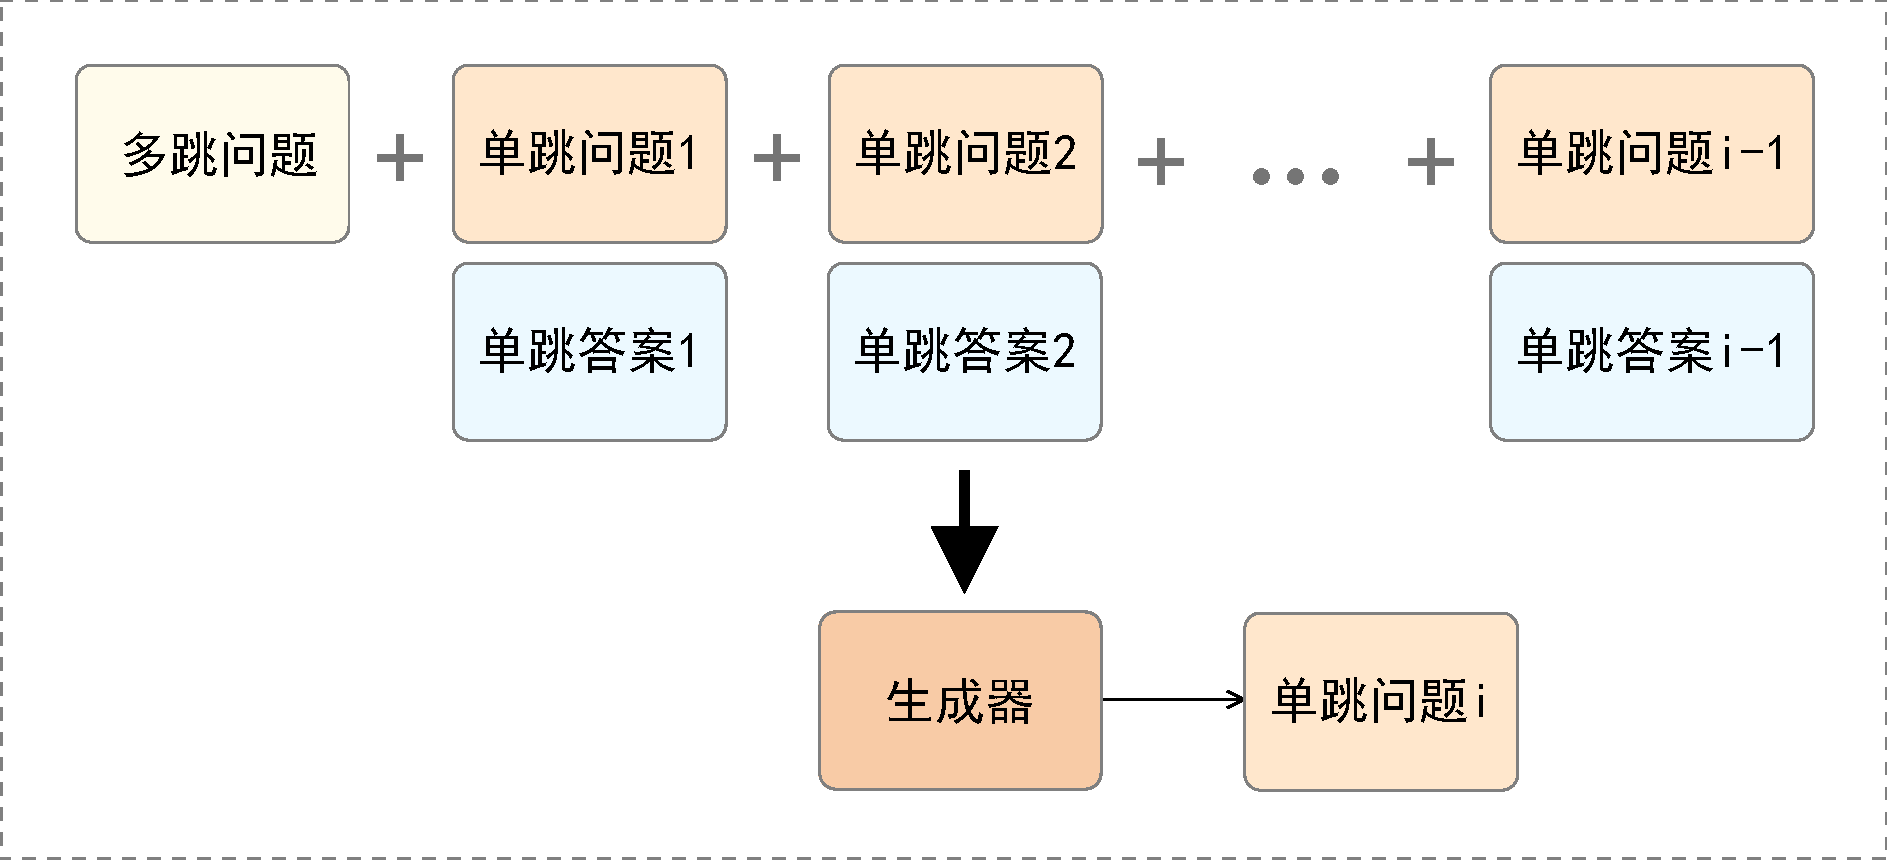
\includegraphics [width=0.8\textwidth] {figure/5-2.pdf}
    \caption{StepDecomposer的问题分解过程} 
    \label{fig:5-2}
\end{figure}



\section{实验及结果分析}

\subsection{实验设置}
% 数据集简介
本章进行了大量实验,主要在多跳多文档阅读理解数据集MuSiQue上进行。
MuSiQue的文章主要来源于英文维基百科,是对一些经典的阅读理解数据集(如SQuAD等)的重构。
该数据集中对于每个问题所给出的相关文档数量要远远大于其他多跳数据集,其中99\%以上的问题都给出了20个可能相关的文档,还有少部分问题是给出了16-19个文档。
MuSiQue包含了2-4跳总共约25k个问题,其中2跳问题占据了绝大多数。
训练集包含了20k个问题。
与以往的多跳阅读理解数据集不同,MuSiQue往往需要给出正确的多跳支持证据才能找到最终答案。
本文还统计了MuSiQue中问题的长度分布,训练集中多跳问题的token数量中位数为18,经过训练好的生成模型将其分解为多个单跳问题后,拼接后的句子的token数量的中位数为28。

% Baseline介绍
本章采用了选择器+问答器架构作为基线模型。
该架构首先对备选文档进行排序,筛选出K个最相关的文档$D_K$\footnote{K是一个超参,通常设定为3,5,或7}。
具体而言,对于给定的问题$Q$,需要判断每个文档$D_i$与$Q$是否相关,训练时使用交叉熵损失。
随后,回答器基于筛选出的文档$D_K$来预测答案及其支持证据。
选择器使用了RoBERTa-large作为预训练语言模型,而回答器则使用了Longformer-large作为预训练语言模型。
在筛选出$K$个相关文档后,回答器使用这些文档来生成答案和支持证据。

% 超参数设定
本章主要使用支持证据F1和答案F1来衡量多跳机器阅读理解模型的性能。

本章基于问题分解技术提出了两个模型SeqDecomposer和StepDecomposer。
在问题分解阶段,本研究使用BART-large\cite{Lewis2019BARTDS}和T5-large\cite{Ni2021SentenceT5SS}进行大部分实验。
在问答阶段,本研究主要使用ALBERT-xxlarge\cite{lan2019albert}和DeBERTaV3-large作为预训练语言模型。
在训练阶段,所有模型的学习率均为1e-5。
在生成阶段,BART模型的batch size为64,epochs为2,T5模型的batch size为16,epochs为2。
在问答阶段,DeBERTa的batch size为2,epochs为3,ALBERT的batch size为1,epochs为2。

\subsection{实验结果和分析}
% 问题分解部分的实验
表~\ref{tab:5-2}~记录了SeqDecomposer的问题分解部分在三个生成指标上的表现。
从表中可以看出,BART-large由于其本身的预训练方式,非常适合做序列到序列生成的任务,因此其在问题分解任务中的表现要优于T5。
因此,本节剩余的关于问题分解的实验都会基于BART-large进行。

\begin{table}[htbp]
    \centering
    \caption{SeqDecomposer的问题分解评价指标。}
    \begin{tabular}{lccc}
    \hline
    & BLEU & METEOR & ROUGE \\
    \hline
    BART-large & \underline{49.4} & \underline{74.2} & 53.0 \\
    % \hline
    T5-large & 49.0 & 73.2 & \underline{53.4} \\
    \hline
    \end{tabular}
    \label{tab:5-2}
\end{table}


此外,本文针对2跳、3跳和4跳的问题,分别统计了各自的生成指标,如表~\ref{tab:5-3}~所示。
不同跳数之间存在明显差异,一方面是因为更高跳数的问题分解难度更大,另一方面是对应的训练数据更少。
由于StepDecomposer的分解方式是在得到了上一问的答案的基础上再进行生成,因此,本文采用将所有单跳问题拼接的方法,评估对应的生成指标。
对比结果如表~\ref{tab:5-4}~所示。
可以看出,StepDecomposer的生成指标略低于SeqDecomposer,原因是融合了问答模型中抽取的一些错误答案。

\begin{table}[htbp]
    \centering
    \caption{使用BART-large的SeqDecomposer在2,3,4跳问题分解上的评价指标}
    \begin{tabular}{lccc}
    \hline
    & BLEU & METEOR & ROUGE \\
    \hline
    2跳 & 53.4 & 77.7 & 56.0 \\
    3跳 & 47.3 & 72.8 & 51.6 \\
    4跳 & 40.7 & 66.1 & 46.3 \\
    \hline
    \end{tabular}
    \label{tab:5-3}
\end{table}

\begin{table}[htbp]
    \centering
    \caption{SeqDecomposer和StepDecomposer的问题分解评价指标对比}
    \begin{tabular}{lccc}
    \hline
    & BLEU & METEOR & ROUGE \\
    \hline
    SeqDecomposer & \underline{49.4} & \underline{74.2} & 53.0 \\
    % \hline
    StepDecomposer & 48.9 & 71.9 & \underline{55.5} \\
    \hline
    \end{tabular}
    \label{tab:5-4}
\end{table}


% 生成指标(5B)混合/2-3-4跳
% 生成(4B-c)seq和step

% 检索器的实验
接下来,本文按照与基线模型相同的方式,训练一个检索器。
对于每个子问题,数据集给定了相应的唯一一个支持文档。
本文的工作在于判断问题与每个文档是否对应,通过计算交叉熵损失,得到得分最高的文档,作为支持文档。
其实验数据如表~\ref{tab:5-5}~所示。
表格中的预训练语言模型都可以做到对文档的高质量检索,即便是参数量更高的模型,相对于BERT-base也不会有明显差异。
表中两列数据的差异在于,是否为文档加上标题。
结果是加标题与否,对最终的性能没有明显影响。

接下来,本文将按照与基线模型相同的方式训练一个检索器。
对于每个子问题,数据集给定了一个相应的唯一支持文档。
本文的工作在于判断问题与每个文档是否对应,并通过计算交叉熵损失得到得分最高的文档作为支持文档。
实验结果如表~\ref{tab:5-5}~所示。
表格中的预训练语言模型都可以实现高质量的文档检索,即便是参数量更高的模型,与BERT-base相比也没有明显差异。
表中两列数据的差异在于是否为文档加上标题。
实验结果表明,加标题与否对最终的性能没有明显影响。

% 检索器ACC(5D)检索器

\begin{table}[htbp]
    \centering
    \caption{检索器的评价指标}
    \begin{tabular}{lcc}
    \hline
    & ACC(无标题) & ACC(有标题) \\
    \hline
    BERT-base & 96.3 & 96.6 \\
    BERT-large & 96.8 & 97.1 \\
    BERT-base & 97.4 & \underline{97.4} \\
    BERT-base & \underline{97.5} & 97.2 \\
    \hline
    \end{tabular}
    \label{tab:5-5}
\end{table}


% 阅读器的实验
此外,本文需要训练一个单跳阅读器。
该阅读器能够在给定单跳问题和支持文档的情况下,利用阅读理解技术从文档中提取答案。
实验结果如表~\ref{tab:5-6}~所示,不同规格的模型的性能表现存在较大差异。
因此,本文的主要实验采用了DeBERTa和ALBERT这两个更优的预训练语言模型。

% 阅读器F1(5C)单跳reader

\begin{table}[htbp]
    \centering
    \caption{阅读器的评价指标}
    \begin{tabular}{lcccc}
    \hline
    & F1(无标题) & F1(有标题) & EM(无标题) & EM(有标题) \\
    \hline
    BERT-base & 64.3 & 61.5 & 57.6 & 54.3 \\
    BERT-large & 73.1 & 72.0 & 65.6 & 64.1 \\
    DeBERTaV3-large & 81.9 & 82.5 & 73.5 & 73.8 \\
    ALBERT-xxlarge & \underline{84.5} & \underline{84.3} & \underline{77.0} & \underline{76.0} \\
    \hline
    \end{tabular}
    \label{tab:5-6}
\end{table}


% 主实验
表~\ref{tab:5-7}~展示了使用BART-large模型进行问题分解,结合DeBERTaV3-large和ALBERT-xxlarge两种模型进行检索与问答阶段的实验结果。
实验结果表明了三个现象。
首先,相对于SeqDecomposer,StepDecomposer在两个评价指标上都略微提升,这表明本文针对问题分解方式的改进取得了一定效果。
由于StepDecomposer存在错误答案积累的情况,这也许是导致该方法并没有特别显著提升的原因。
% 尽管StepDecomposer在直觉上生成问题的方式会比SeqDecomposer更合理,但是由于其错误答案的积累,导致其最终性能与SeqDecomposer相差无几。
其次,在检索和问答阶段中,无论采用DeBERTaV3还是ALBERT的架构,都没有表现出明显的性能差异。
这表明,模型的整体架构起着关键作用,而不是单个环节的模型本身的能力。
最后,在支持证据的F1指标方面,与选择器和回答器的基线模型相比,本章提出的SeqDecomposer和StepDecomposer均有显著的提升,而在答案的F1指标方面略有下降。
其中,SeqDecomposer在支持证据的F1方面的提升最高达6.7,最低为5.0,在答案的F1方面的下降最高达3.7,最低为1.5。
StepDecomposer在支持证据的F1方面的提升最高达7.9,最低为7.5,在答案的F1方面的下降最高达2.2,最低为1.5。
这与模型的初衷相符。
无论是SeqDecomposer还是StepDecomposer,都希望通过将多跳问题分解为单跳问题的形式,找到每一跳问题对应的支持文档,因此它们的支持文档的F1值会更高。
而基线模型中提出的选择器和回答器的模式偏向于直接将多跳问题和备选文档输入神经网络,从而快速获得答案,因此该方法更倾向于答案抽取。

% 主实验(4B-e)seq和step 过时
% 主实验(3A-e)seq和step
% 基线(3C-a3)第一名检索方法

\begin{table}[htbp]
    \centering
    \caption{SeqDecomposer和StepDecomposer的实验性能}
    \begin{tabular}{lcccc}
    \hline
    模型 & 支持 F1 & 支持 EM & 答案 F1 & 答案 EM \\
    \hline
    % \multicolumn{5}{c}{基线} \\
    \multicolumn{5}{l}{基线} \\
    % \hline
    RoBERTa-large \& Longformer-large & 75.2 & - & \underline{52.3} & - \\
    \hline
    % \multicolumn{5}{c}{SeqDecomposer} \\
    \multicolumn{5}{l}{SeqDecomposer模型} \\
    % \hline
    DeBERTaV3 \& DeBERTaV3 & 80.2 & 49.9 & 49.6 & 39.8 \\
    DeBERTaV3 \& ALBERT & 80.5 & 50.7 & 48.6 & 38.1 \\
    ALBERT \& DeBERTaV3 & 81.8 & 51.1 & \underline{50.8} & \underline{41.1} \\
    ALBERT \& ALBERT & \underline{81.9} & \underline{51.8} & 49.7 & 39.6 \\
    \hline
    % \multicolumn{5}{c}{StepDecomposer} \\
    \multicolumn{5}{l}{StepDecomposer模型} \\
    % \hline
    DeBERTaV3 \& DeBERTaV3 & 82.7 & 56.1 & 50.7 & \underline{42.1} \\
    DeBERTaV3 \& ALBERT & 83.0 & \underline{57.8} & \underline{50.8} & 40.3 \\
    ALBERT \& DeBERTaV3 & 83.0 & 56.7 & 50.2 & 41.6 \\
    ALBERT \& ALBERT & \underline{83.1} & 56.3 & 50.1 & 39.9 \\
    \hline
    \end{tabular}
    \label{tab:5-7}
\end{table}



\section{本章小结}

本章提出了一种基于问题分解技术,用以处理多跳阅读理解任务的方法,并改善模型搜寻支持证据的能力。
该方法包括SeqDecomposer和StepDecomposer两种类型,两者都将复杂的多跳问题分解为多个简单的单跳问题,然后依次完成检索和阅读理解任务。
实验结果和分析表明,该方法在捕获证据文档的能力方面有显著的提升。
不过,本章还未对模型进行全方位的探索。
因此,未来的研究将考虑应用大型模型中思维链的方式,对问题分解进行更细致的研究。


